\documentclass[a4paper]{article}
\usepackage{xcolor}%颜色支持
\definecolor{vscode_backgroundcolor}{rgb}{0.15, 0.2, 0.22}
\definecolor{vscode_localvariablecolor}{rgb}{0.93,1,0.89}
\definecolor{vscode_keywordcolor}{rgb}{0.57, 0.52, 1}
\definecolor{vscode_commentcolor}{rgb}{0.2, 0.34, 0.45}
\definecolor{vscode_stringcolor}{rgb}{0.76, 0.91, 0.55}
\definecolor{vscode_semicolomncolor}{rgb}{1,1,1}
\definecolor{vscode_headerfilecolor}{rgb}{0.93,1,0.89}
\definecolor{vscode_linenumbercolor}{rgb}{0.2, 0.34, 0.45}
\definecolor{vscode_numbercolor}{rgb}{0.96, 0.54, 0.42}
\definecolor{vscode_parametercolor}{rgb}{0.96, 0.54, 0.42}
\definecolor{vscode_operatorcolor}{rgb}{0.53, 0.85, 0.99}
\definecolor{vscode_callablecolor}{rgb}{0.36, 0.62, 0.96}
\definecolor{vscode_rulecolor}{rgb}{0.22, 0.28, 0.31}
\definecolor{vscode_classcolor}{rgb}{1, 0.8, 0.42}
\definecolor{vscode_selfcolor}{rgb}{0.97, 0.31, 0.43}

\usepackage{listings}%高亮代码块支持
\lstloadlanguages{Python}
\lstdefinestyle{MyPython}{
    extendedchars=false,
    numbers=left,
    firstnumber=auto,
    frame=leftline,
    backgroundcolor=\color{vscode_backgroundcolor},
    framerule=0.5ex,
    columns=fixed,
    language=Python,
    basicstyle=\ttfamily\color{vscode_localvariablecolor},
    % commentstyle=\color{vscode_commentcolor},
    keywordstyle=\color{vscode_keywordcolor},
    stringstyle=\color{vscode_stringcolor},
    morecomment=[l][\color{vscode_commentcolor}]{\#},
    morecomment=[s][\color{vscode_headerfilecolor}]{"""}{"""},
    numberstyle=\code\color{vscode_linenumbercolor},
    morekeywords={
        None,
        True,
        yield,
        False,
    },
    alsoletter={
        =+-*<>^&
        % ;0123456789
        % 0,1,2,3,4,5,6,7,8,9
    },%把;设置为可以识别的letter,也可以使用otherkeywords,但是无法将其和其他keywords区分开来
    emph={=,+,-,*,>,<,<<,>>,^,+=,&},emphstyle=\color{vscode_operatorcolor},
    % alsoletter={!,\%,&,*,-,+,=,/,<,>},
    emph={[2]%一些全局的函数和可调用对象
    DataFrame,
    arange,
    interp2d,
    f,
    subplots,
    contour,
    show,
    clabel,
    getWalls,
    AnyFoodSearchProblem,
    print,
    range,
    scatter,
    spline,
    UnivariateSpline,
    diff,
    len
    },emphstyle={[2]\color{vscode_callablecolor}},
    emph={[5]
    self},emphstyle={[5]\color{vscode_selfcolor}},
    % emphstyle={[3]\color{vscode_parametercolor}}
     % emph={[3]0,1,2,3,4,5,6,7,8,9},emphstyle={[3]\color{yellow}},
    tabsize=4,
    rulecolor=\color{vscode_rulecolor},
    breaklines=true,
}
\lstset{
    style=MyPython,
}
\usepackage[
    fontset=none,%设置中文支持,并自定义字体
    zihao=5,%默认字号为五号
    heading=true,%允许后续自定义标题样式
    scheme=chinese,%自动将文档样式中文化,例如图标标题
    punct=quanjiao,%全角式标点符号
    space=auto,%中文后接换行不会添加空格,但是英文会添加空格,需要用%手动取消
    linespread=1.3,%行距倍数是1.3
    autoindent=true,%自动缩进两个中文宽度
    ]{ctex}
\ctexset{
    % tday=small,%小写样式的日期
    contentsname={目录},
    listfigurename={插图},
    listtablename={表格},
    figurename={图},
    tablename={表},
    abstractname={摘要},
    indexname={索引},
    appendixname={附录},
    bibname={参考文献},
    proofname={证明},
    % refname={参考文献},%只适用于beamer
    % algorithmname={算法},
    % continuation={(续)},%beamer续页的标识
    section={
        format+ = \Large\heiti\raggedright,
        name = {,\num\textbf{.}\hspace{1ex}},
        number={\num\thesection},
        nameformat={},
        numberformat={},
        aftername={},
        titleformat={},
        aftertitle={},
        runin=false,%对section级以下有用,标题是否和正文在同一段上
        beforeskip={3.5ex plus 1ex minus .2ex},%标题前垂直间距
        afterskip={2.3ex plus .2ex}%标题后垂直间距
    },
    subsection={
        format+ = \large\heiti\raggedright,
        name = {,\num\textbf{.}\hspace{1ex}},
        number={\num\thesubsection},
        nameformat={},
        numberformat={},
        aftername={},
        titleformat={},
        aftertitle={},
        runin=false,%对section级以下有用,标题是否和正文在同一段上
        beforeskip={3.5ex plus 1ex minus .2ex},%标题前垂直间距
        afterskip={2.3ex plus .2ex}%标题后垂直间距
    },
    subsubsection={
        format+ = \normalsize\heiti\raggedright,
        name = {,\num\textbf{.}\hspace{1ex}},
        number={\num\thesubsubsection},
        nameformat={},
        numberformat={},
        aftername={},
        titleformat={},
        aftertitle={},
        runin=false,%对section级以下有用,标题是否和正文在同一段上
        beforeskip={3.5ex plus 1ex minus .2ex},%标题前垂直间距
        afterskip={2.3ex plus .2ex}%标题后垂直间距
    },
    }

% 中文默认字体: 思源宋体,粗体为思源宋体半粗体,斜体为方正楷体_GBK
\setCJKmainfont{Source Han Serif SC}[BoldFont={Source Han Serif SC Heavy}, ItalicFont=FZKai-Z03S]
% 中文无衬线字体:思源黑体,粗体为思源黑体粗体
\setCJKsansfont{Source Han Sans CN}[BoldFont={Source Han Sans CN Heavy}]
% 中文等宽字体:微软雅黑light
\setCJKmonofont{Microsoft YaHei}[ItalicFont={Microsoft YaHei Light}]

\newCJKfontfamily\songti{Source Han Serif SC}[BoldFont={Source Han Serif SC Heavy}]
\newCJKfontfamily\xbsong{Source Han Serif SC SemiBold} % 小标宋
\newCJKfontfamily\dbsong{Source Han Serif SC Bold} % 大标宋
\newCJKfontfamily\cusong{Source Han Serif SC Heavy} % 粗宋
\newCJKfontfamily\heiti{Source Han Sans CN}[BoldFont={Source Han Sans CN Heavy}]
\newCJKfontfamily\dahei{Source Han Sans CN Medium} % 大黑
\newCJKfontfamily\cuhei{Source Han Sans CN Heavy} % 粗黑
\newCJKfontfamily\fangsong{FZFangSong-Z02S}
\newCJKfontfamily\kaiti{FZKai-Z03S}[ItalicFont={Microsoft YaHei Light}]%这个斜体只是用于lstlisting环境中的中文注释
% \newCJKfontfamily\kaiti{FZKai-Z03S}[ItalicFont={FZZJ-LZXTFSJW}]%这个斜体只是用于lstlisting环境中的中文注释
\setsansfont{Arial}
\setmonofont{Consolas}%设置西文等宽字体
\newfontfamily\code{Consolas}
\newfontfamily\num{Arial}

\usepackage{geometry}%设置整体页面布局
\geometry{a4paper}
\geometry{left=2cm,right=2cm,top=2.54cm,bottom=2.54cm}%word常规页边距
% \geometry{left=1.27cm,right=1.27cm,top=1.27cm,bottom=1.27cm}%word窄页边距
\setlength{\headheight}{13pt}%避免warning


\usepackage{fancyhdr}%必须在geometry包之后使用
\fancyhf{}
\makeatletter
\lhead{{\dahei \@title}}%可以使用thepage,CTEXthechapter,CTEXthesection
\makeatother
\rhead{\textbf{\num- \thepage{} -}}
\renewcommand\headrulewidth{1.5pt}%设置眉头宽度
\pagestyle{fancy}

\usepackage[ruled,algosection,lined,longend,fillcomment,linesnumbered,resetcount,titlenotnumbered]{algorithm2e}
%参数解释:带框,按section编码,有竖线,end前带if等关键词,注释占满整行,代码部分编号(不包括输入输出、注释),每个代码块重新编号,可以调用TitleOfAlgo来打印算法标题但不作为单独的算法编码
%附带algorithm,function,procedure环境,其中function,procedure环境下,设置caption时,必须带有(),
%()之前的字符会被视为宏,可以在接下来的部分用\名字()来调用,所以推荐辅助函数用function,其中的某些展开部分用procedure,描述算法整体使用algorithm
\DontPrintSemicolon
\SetAlCapSkip{2ex}
\SetSideCommentRight
\SetFillComment
\newcommand{\forcond}{$i=0$ \KwTo $n$}
\SetKw{downto}{downto}%自定义关键词
\SetKwFunction{funcmacro}{text}%自定义函数名,实际上function环境是在定义宏的同时说明了其内容
\SetKwProg{procedmacro}{text}{begin text}{end text}%自定义步骤,和function类似,但是后面两个参数可以设置开始和结尾的标志,和if等环境一样
\SetKwData{datamacro}{text}%可以用于突出特殊的变量,例如数据结构
\SetKwFunction{FRecurs}{FnRecursive}
\SetKwProg{Fn}{Function}{begin}{end}

\usepackage[strict]{changepage}
\usepackage{framed}%色块支持
\definecolor{formalshade}{rgb}{0.95,0.95,1} % 文本框颜色
% ------------------******-------------------
% 注意行末需要把空格注释掉,不然画出来的方框会有空白竖线
\newenvironment{formal}{%
\def\FrameCommand{%
\hspace{1pt}%
{\color{DarkBlue}\vrule width 2pt}%
{\color{formalshade}\vrule width 4pt}%
\colorbox{formalshade}%
}%
\MakeFramed{\advance\hsize-\width\FrameRestore}%
\noindent\hspace{-4.55pt}% disable indenting first paragraph
\begin{adjustwidth}{}{7pt}%
\vspace{2pt}\vspace{2pt}%
}
{%
\vspace{2pt}\end{adjustwidth}\endMakeFramed%
}

% 自定义标题格式
\makeatletter
\renewcommand{\maketitle}{
  \begin{center}
    \thispagestyle{fancy}
    {\quad}\\
    \vspace{0.1\textheight}
    {\huge\sffamily\bfseries\@title}\\ % 标题字体大小、粗体、颜色
    \vspace{2em} % 标题与作者名之间的垂直空间
    {\large\sffamily\@author} \\
  \end{center}
}
\makeatother

\usepackage{graphicx}

\title{作业{\hspace{1ex}}Chapter 3}
\author{姓名:范潇{\quad}学号:2254298{\quad}日期:\today}
\date{}
\begin{document}
\maketitle
\section{(5.2)}
我使用Python完成了对本题的求解。

\begin{lstlisting}[emph={[3]columns,index,kind,inline,fontsize},emphstyle={[3]\color{vscode_parametercolor}},emph={[4]SearchProblem,Callable,Node,Reached,Any,Tuple,List,FoodSearchProblem},emphstyle={[4]\color{vscode_classcolor}}]
import numpy as np
import pandas as pd
import matplotlib.pyplot as plt
from scipy import interpolate
data = [
    [370, 470, 550, 600, 670, 690, 670, 620, 580, 450, 400, 300, 100, 150, 250],
    [510, 620, 730, 800, 850, 870, 850, 780, 720, 650, 500, 200, 300, 350, 320],
    [650, 760, 880, 970, 1020, 1050, 1020, 830, 800, 700, 300, 500, 550, 480, 350],
    [740, 880, 1080, 1130, 1250, 1280, 1230, 1040, 900, 500, 700, 780, 750, 650, 550],
    [830, 980, 1180, 1320, 1450, 1420, 400, 1300, 700, 900, 850, 810, 380, 780, 750],
    [880, 1060, 1230, 1390, 1500, 1500, 1400, 900, 1100, 1060, 950, 870, 900, 936, 950],
    [910, 1090, 1270, 1500, 1200, 1100, 1350, 1450, 1200, 1150, 1010, 880, 1000, 1050, 1100],
    [950, 1190, 1370, 1500, 1200, 1100, 1550, 1600, 1550, 1380, 1070, 900, 1050, 1150, 1200],
    [1430, 1450, 1460, 1500, 1550, 1600, 1550, 1600, 1600, 1600, 1550, 1500, 1500, 1550, 1550],
    [1420, 1430, 1450, 1480, 1500, 1550, 1510, 1430, 1300, 1200, 980, 850, 750, 550, 500],
    [1380, 1410, 1430, 1450, 1470, 1320, 1280, 1200, 1080, 940, 780, 620, 460, 370, 350],
    [1370, 1390, 1410, 1430, 1440, 1140, 1110, 1050, 950, 820, 690, 540, 380, 300, 210],
    [4800, 1370, 1390, 1400, 1410, 960, 940, 880, 800, 690, 570, 430, 290, 210, 150]
]
data = pd.DataFrame(data, columns=range(0, 6000, 400), index=range(0, 5200, 400))
x = np.arange(0, 4850, 50)
y = np.arange(0, 5650, 50)
f = interpolate.interp2d(data.columns, data.index, data, kind='linear')
z = f(x, y)
fig, ax = plt.subplots()
contour = ax.contour(x, y, z)
ax.clabel(contour, inline=True, fontsize=10)
plt.show()
z = pd.DataFrame(z, columns=x, index=y)
z.to_csv('height.csv')
\end{lstlisting}
得到的等高图如下图所示,得到的高程数据存储在文件height.csv中。
\begin{figure}[!h]
    \centering
    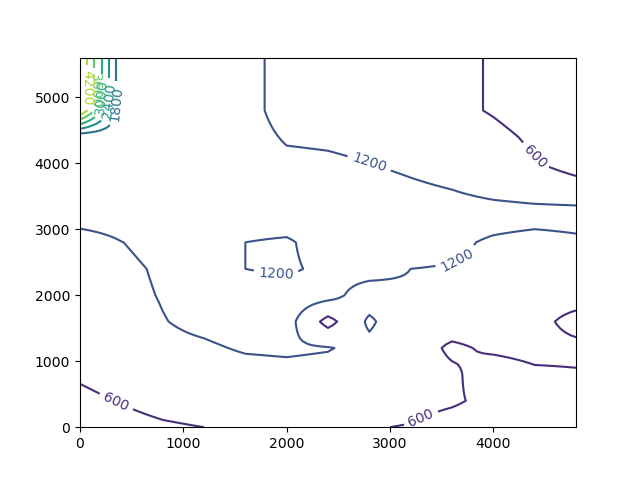
\includegraphics[width=\textwidth]{Figure_1.png}
    \caption{等高图}
\end{figure}
\newpage
\section{(5.3)}
我使用Python完成了对本题的求解。
\begin{lstlisting}[emph={[3]columns,index,kind,inline,fontsize,x,y,a,b},emphstyle={[3]\color{vscode_parametercolor}},emph={[4]SearchProblem,Callable,Node,Reached,Any,Tuple,List,FoodSearchProblem},emphstyle={[4]\color{vscode_classcolor}}]
import numpy as np
from scipy.optimize import curve_fit

def f(x,a,b):
    return a*np.e**(b*x)

x = range(1,9)
y = [15.3, 20.5,27.4,36.6,49.1,65.6,87.87,117.6]

initial_guess = [15,1]
fit_params, covariance = curve_fit(f,x,y,initial_guess)

a_fit,b_fit = fit_params
print(a_fit,b_fit)
\end{lstlisting}
得到的输出为11.425066497697129和0.2914239509980085。
\newpage
\section{(5.4)}
我使用Python完成了对本题的求解。

思路是利用题中所给的数据点(不包括泵水阶段)来拟合出各个时间与水位之间的函数关系,然后通过差分来得到水位差值关于时间的函数,乘以常数后便得到
流量的近似函数。
\begin{lstlisting}[emph={[3]columns,index,kind,inline,fontsize,x,y,a,b},emphstyle={[3]\color{vscode_parametercolor}},emph={[4]SearchProblem,Callable,Node,Reached,Any,Tuple,List,FoodSearchProblem},emphstyle={[4]\color{vscode_classcolor}}]
import numpy as np
import matplotlib.pyplot as plt
from  scipy.interpolate import UnivariateSpline
x1 = [0,3316,6635,10619,13937,17921,21240,25223,28543,32284]
y1 = [3175,3110,3054,2994,2947,2892,2850,2795,2752,2697]
x2 = [39435,43318,44636,49953,53936,57254,60574,64554,68535,71854,75021]
y2 = [3550,3445,3350,3260,3167,3087,3012,2927,2842,2767,2697]
x3 = [85968,89953,93270]
y3 = [3475,3397,3340]
spline = UnivariateSpline(x1+x2+x3,y1+y2+y3)
x = range(0,89953)
y = spline(x)
plt.scatter(x = range(len(np.diff(y))),y=np.diff(y))
\end{lstlisting}
得到的输出如下图所示:
\begin{figure}[!hb]
    \centering
    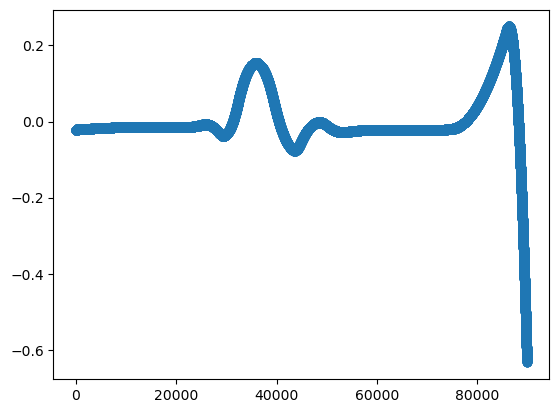
\includegraphics{output.png}
    \caption{时间-水位差值关系}
\end{figure}

可以看到插值得到的函数在右端偏差较大,但是由于假设(4),只需取$[0,86400]$内的函数即可,而在该范围内的差异偏差较小。

在此基础上,只需乘以常数$\frac{E^2\pi}{4}$即可得到流量函数$f(t)$。
\newpage
\end{document}